\documentclass{oblivoir}
\usepackage{amsmath,amssymb,amsthm,kotex,paralist,kswrapfig}

\usepackage[skipabove=10pt,innertopmargin=10pt]{mdframed}

\usepackage{tabto,pifont}
\TabPositions{0.2\textwidth,0.4\textwidth,0.6\textwidth,0.8\textwidth}
\newcommand\tabb[5]{\par\bigskip\noindent
\ding{172}\:{\ensuremath{#1}}
\tab\ding{173}\:\:{\ensuremath{#2}}
\tab\ding{174}\:\:{\ensuremath{#3}}
\tab\ding{175}\:\:{\ensuremath{#4}}
\tab\ding{176}\:\:{\ensuremath{#5}}}

\usepackage{enumitem}
\setlist[enumerate]{label=(\arabic*)}

\newcounter{num}
\newcommand{\defi}[1]
{\noindent\refstepcounter{num}\textbf{정의 \arabic{num}) #1}\par\noindent}
\newcommand{\theo}[1]
{\noindent\refstepcounter{num}\textbf{정리 \arabic{num}) #1}\par\noindent}
\newcommand{\exam}[1]
{\bigskip\bigskip\noindent\refstepcounter{num}\textbf{예시 \arabic{num}) #1}\par\noindent}
\newcommand{\prob}[1]
{\bigskip\bigskip\noindent\refstepcounter{num}\textbf{문제 \arabic{num}) #1}\par\noindent}
\newcommand{\proo}
{\bigskip\textsf{증명)}\par}

\newcommand{\ans}{
{\par\raggedleft\textbf{답 : (\qquad\qquad\qquad\qquad\qquad\qquad)}\par}\bigskip\bigskip}
\newcommand\an[1]{\par\bigskip\noindent\textbf{문제 #1)}\\}

\newcommand{\pb}[1]%\Phantom + fBox
{\fbox{\phantom{\ensuremath{#1}}}}

\newcommand\ba{\,|\,}

\let\oldsection\section
\renewcommand\section{\clearpage\oldsection}

\newenvironment{talign}
 {\let\displaystyle\textstyle\align}
 {\endalign}
\newenvironment{talign*}
 {\let\displaystyle\textstyle\csname align*\endcsname}
 {\endalign}

%%%%
\begin{document}

\title{준영 : 06 수열(4)}
\author{}
\date{\today}
\maketitle
\tableofcontents
\newpage

%%
\section{수열의 귀납적 정의(1)}
%
\exam{}
첫째항이 \(1\)이고 공차가 \(2\)인 등차수열
\[1,\quad3,\quad5,\quad7,\quad\cdots\]
는 일반항 \(a_n=1+(n-1)\cdot 2=2n-1\)로 나타내기도 하지만 첫째항 \(1\)부터 차례로 일정한 수 \(2\)를 더해서 얻어지는 수열이므로
\[a_1=1,\quad a_{n+1}=a_n+2\:\:(n=1,2,3,\cdots)\]
와 같이 첫째항과 이웃하는 항들 사이의 관계식을 이용하여 수열을 정의하기도 한다.

\begin{mdframed}
%
\defi{수열의 귀납적 정의}
일반적으로 \(a_1\)의 값과 \(a_n\)에서 \(a_{n+1}\)을 구할 수 있는 관계식이 주어지면 수열 \(\{a_n\}\)의 모든 항 \(a_1\), \(a_2\), \(a_3\), \(\cdots\)이 정해진다.
이와 같이 첫째항과 이웃하는 항들 사이의 관계식으로 수열을 정의하는 것을 수열의 \textbf{귀납적 정의}라고 한다.
이때, 이웃하는 항들 사이의 관계식을 \textbf{점화식}이라고 한다.
\end{mdframed}

\exam{}
\(a_1=1\),\:\:\(a_{n+1}=2a_n+1\:\:(n=1,2,3,\cdots)\)로 정의된 수열 \(\{a_n\}\)에서 제 4항을 구하면
\[
\begin{aligned}
n=1\text{을 대입 : }	&a_2=2\cdot1+1=3\\
n=2\text{을 대입 : }	&a_3=2\cdot3+1=7\\
n=3\text{을 대입 : }	&a_4=2\cdot7+1=15
\end{aligned}
\]
따라서 수열 \(\{a_n\}\)의 제4항은 \(15\)이다.

%
\prob{}
다음과 같이 귀납적으로 정의된 수열 \(\{a_n\}\)의 제5항을 구하여라.
\begin{enumerate}
\item
\(a_1=2\),~~ \(a_{n+1}=a_n+3\)
\item
\(a_1=2\),~~ \(a_{n+1}=\frac12a_n\)
\end{enumerate}

%
\prob{}\label{iterating}
다음과 같이 귀납적으로 정의된 수열 \(\{a_n\}\)의 제5항을 구하여라.
\begin{enumerate}
\item\label{iterating_sum}
\(a_1=3\),~~ \(a_{n+1}=a_n+n\)~\((n=1,2,3,\cdots)\)
\begin{mdframed}
\vspace{0.1\textheight}
\end{mdframed}
\ans
\item\label{iterating_multiplication}
\(a_1=1\),~~ \(a_{n+1}=\frac{n+2}{n}a_n\)~\((n=1,2,3,\cdots)\)
\begin{mdframed}
\vspace{0.1\textheight}
\end{mdframed}
\ans
\item\label{iterating_difference}
\(a_1=1\),~~ \(a_{n+1}=3a_n+2\)~\((n=1,2,3,\cdots)\)
\begin{mdframed}
\vspace{0.1\textheight}
\end{mdframed}
\ans
\end{enumerate}

%
\prob{}
다음과 같이 귀납적으로 정의된 수열 \(\{a_n\}\)에서 \(a_5+a_{10}\)의 값을 구하여라.
\begin{enumerate}
\item\label{Fibonacci}
\(a_1=1\),~~\(a_2=1\),~~\(a_{n+2}=a_n+a_{n+1}\)~\((n=1,2,3,\cdots)\)
\begin{mdframed}
\vspace{0.2\textheight}
\end{mdframed}
\ans
\item
\(a_1=1\),~~\(a_2=2\),~~\(a_{n+2}=a_n+1\)~\((n=1,2,3,\cdots)\)
\begin{mdframed}
\vspace{0.2\textheight}
\end{mdframed}
\ans
\end{enumerate}

위 문제에서 \ref{Fibonacci}의 수열은 \textbf{피보나치 수열}이라고 불린다.

%\begin{mdframed}
%%
%\theo{등차수열과 등비수열의 귀납적 정의}
%수열 \(\{a_n\}\)에 대하여 이웃하는 항 사이의 관계식이
%\begin{enumerate}
%\item
%\(a_{n+1}-a_n=d\)이면 공차가 \(d\)인 등차수열이다.
%\item
%\(2a_{n+1}=a_n+a_{n+2}\)이면 등차수열이다.
%\item
%\(\frac{a_{n+1}}{a_n}=r\)이면 공비가 \(r\)인 등비수열이다.
%\item
%\({a_{n+1}}^2=a_na_{n+2}\)이면 등비수열이다.
%\end{enumerate}
%\end{mdframed}

\clearpage
%
\exam{}
다음과 같이 귀납적으로 정의된 수열의 일반항을 구하여라.
\begin{enumerate}
\item
\(a_1=5\),~~\(a_{n+1}=a_n+8\)~\((n=1,2,3,\cdots)\)
\begin{mdframed}[skipabove=-1pt]
\(a_{n+1}-a_n=8\)에서 공차가 \(8\)인 등차수열임을 알 수 있다.
첫항은 \(a=5\)이므로
\[a_n=5+(n-1)8=8n-3\]
\end{mdframed}
{\par\raggedleft\textbf{답 : \(a_n=8n-3\)\quad}\par}\bigskip
\item
\(a_1=2\),~~\(a_2=6\),~~\(2a_{n+1}=a_{n+2}+a_n\)~\((n=1,2,3,\cdots)\)
\begin{mdframed}[skipabove=-1pt]
\(2a_{n+1}=a_{n+2}+a_n\)에서 \(a_{n+1}\)은 \(a_n\)과 \(a_{n+2}\)의 등차중항이다.
따라서 인접한 세 항은 등차수열을 이루고, 전체 수열도 등차수열임을 알 수 있다.
첫항은 \(a=2\)이고 공차는 \(d=a_2-a_1=4\)이므로
\[a_n=2+(n-1)4=4n-2\]
\end{mdframed}
{\par\raggedleft\textbf{답 : \(a_n=4n-2\)\quad}\par}\bigskip
\item
\(a_1=1\),~~\(a_{n+1}=2a_n\)~\((n=1,2,3,\cdots)\)
\begin{mdframed}[skipabove=-1pt]
\(\frac{a_{n+1}}{a_n}=2\)에서 공비가 \(2\)인 등비수열임을 알 수 있다.
첫항은 \(a=1\)이므로
\[a_n=1\cdot2^{n-1}=2^{n-1}\]
\end{mdframed}
{\par\raggedleft\textbf{답 : \(a_n=2^{n-1}\)\quad}\par}\bigskip
\item
\(a_1=4\),~~\(a_2=6\),~~\({a_{n+1}}^2=a_na_{n+2}\)~\((n=1,2,3,\cdots)\)
\begin{mdframed}[skipabove=-1pt]
\({a_{n+1}}^2=a_na_{n+2}\)에서 \(a_{n+1}\)은 \(a_n\)과 \(a_{n+2}\)의 등비중항이다.
따라서 인접한 세 항은 등차수열을 이루고, 전체 수열도 등차수열임을 알 수 있다.
첫항은 \(a=4\)이고 공차는 \(d=a_2\div a_1=\frac32\)이므로
\[a_n=4\times\left(\frac32\right)^{n-1}\]
\end{mdframed}
{\par\raggedleft\textbf{답 : \(a_n=4\times\left(\frac32\right)^{n-1}\)\quad}\par}\bigskip
\end{enumerate}

%
\prob{}
다음과 같이 귀납적으로 정의된 수열의 일반항을 구하여라.
\begin{enumerate}
\item
\(a_1=1\),~~ \(a_{n+1}-a_n=5\)~\((n=1,2,3,\cdots)\)
\begin{mdframed}[skipabove=-2pt]
\vspace{0.11\textheight}
\end{mdframed}
{\par\raggedleft\textbf{답 : \(a_n=\)\qquad\qquad\qquad\qquad}\par}\bigskip
\item
\(a_1=4\),~~ \(a_2=2\),~~ \(\displaystyle a_{n+1}=\frac{a_{n+2}+a_n}2\)~~\((n=1,2,3,\cdots)\)
\begin{mdframed}[skipabove=-2pt]
\vspace{0.11\textheight}
\end{mdframed}
{\par\raggedleft\textbf{답 : \(a_n=\)\qquad\qquad\qquad\qquad}\par}\bigskip
\item
\(a_1=4\),~~ \(\displaystyle\frac{a_{n+1}}{a_n}=-2\)~~\((n=1,2,3,\cdots)\)
\begin{mdframed}[skipabove=-2pt]
\vspace{0.11\textheight}
\end{mdframed}
{\par\raggedleft\textbf{답 : \(a_n=\)\qquad\qquad\qquad\qquad}\par}\bigskip
\item
\(a_1=\frac13\),~~ \(a_2=1\),~~ \(a_{n+1}=\sqrt{a_na_{n+2}}\)~~\((n=1,2,3,\cdots)\)
\begin{mdframed}[skipabove=-2pt]
\vspace{0.11\textheight}
\end{mdframed}
{\par\raggedleft\textbf{답 : \(a_n=\)\qquad\qquad\qquad\qquad}\par}\bigskip
\end{enumerate}

%%
\section{수열의 귀납적 정의(2)}

%
\exam{}
문제 \ref{iterating}의 \ref{iterating_sum}, \ref{iterating_multiplication}, \ref{iterating_difference}의 일반항을 구해보자.
\begin{enumerate}
%
\item
\(a_1=3\),~~ \(a_{n+1}=a_n+n\)
\begin{mdframed}
점화식의 \(n\)에 \(1\), \(2\), \(3\), \(\cdots\), \(n\)을 차례로 대입하여 나열하면
\begin{align*}
a_2=&\:a_1+1\\
a_3=&\:a_2+2\\
a_4=&\:a_3+3\\
&\vdots\\
a_n=&\:a_{n-1}+(n-1)
\end{align*}
이다.
이 식들을 모두 더하면
%\[a_2+a_3+a_4+\cdots+a_n=a_1+a_2+a_3+\cdots+a_{n-1}+(1+2+3+\cdots+n)\]
%이고 중복된 항들을 지우면
\begin{align*}
a_n
&=a_1+(1+2+3+\cdots+(n-1))\\
&=a_1+\sum_{k=1}^{n-1}k=3+\frac{n(n-1)}2\\
&=\frac{n^2-n+6}2
\end{align*}
이다.
\end{mdframed}
{\par\raggedleft\textbf{답 : \(a_n=\frac{n^2-n+6}2\)\quad}\par}\bigskip

%
\clearpage
\item
\(a_1=1\),~~ \(a_{n+1}=\frac{n+2}{n}a_n\)
\begin{mdframed}
점화식의 \(n\)에 \(1\), \(2\), \(3\), \(\cdots\), \(n\)을 차례로 대입하여 나열하면
\begin{talign*}
\textstyle
a_2=&\:\frac31a_1\\
a_3=&\:\frac42a_2\\
a_4=&\:\frac53a_3\\
a_5=&\:\frac64a_3\\
&\vdots\\
a_{n-1}=&\:\frac{n}{n-2}a_{n-2}\\
a_n=&\:\frac{n+1}{n-1}a_{n-1}
\end{talign*}
이다.
이 식들을 모두 곱하면
%\[a_2a_3a_4\cdots a_n=a_1a_2a_3\cdots a_{n-1}
%\times\frac31\times\frac42\times\frac53\times\frac64\times\cdots\times\frac{n+1}{n-1}\times\frac{n+2}n\]
%이고 중복된 항들을 지우고 약분하면
\begin{talign*}
\textstyle
a_n&=a_1\times\frac31\times\frac42\times\frac53\times\frac64\times\cdots\times\frac{n}{n-2}\times\frac{n+1}{n-1}\\
&=a_1\times\frac{n(n+1)}{1\times2}\\
&=\frac{n(n+1)}2
\end{talign*}
이다.
\end{mdframed}
{\par\raggedleft\textbf{답 : \(a_n=\frac{n(n+1)}2\)\quad}\par}\bigskip

%
\clearpage
\item
\(a_1=1\),~~ \(a_{n+1}=3a_n+2\)
\begin{mdframed}
주어진 점화식
\[a_{n+1}=3a_n+2\]
은
\[a_{n+1}+k=3(a_n+k)\]
꼴로 만들 수 있다.
두 식을 비교해보면 \(2k=2\)이므로 \(k=1\)이고
\[a_{n+1}+1=3(a_n+1)\]
이다.
\(b_n=a_n+1\)을 만족시키는 수열 \(\{b_n\}\)을 생각하면
\[b_{n+1}=3b_n\]
이므로 \(\{b_n\}\)은 공비가 3인 등비수열이다.
\(b_1=a_1+1=1+1=2\)이므로
\[b_n=2\cdot3^{n-1}\]
이고
\[a_n+1=2\cdot3^{n-1}\]
이다.
따라서
\[a_n=2\cdot3^{n-1}-1\]
이다.
\end{mdframed}
{\par\raggedleft\textbf{답 : \(a_n=2\cdot3^{n-1}-1\)\quad}\par}\bigskip
\end{enumerate}
\clearpage

%
\prob{}
다음과 같이 귀납적으로 정의된 수열의 일반항을 구하여라.
\begin{enumerate}
\item
\(a_1=1\), \(a_{n+1}=a_n+4n\)
\begin{mdframed}
\vspace{0.8\textheight}
\end{mdframed}
{\par\raggedleft\textbf{답 : \(a_n=\)\qquad\qquad\qquad\qquad}\par}\bigskip
\clearpage
\item
\(a_1=1\), \(a_{n+1}=2^na_n\)
\begin{mdframed}
\vspace{0.8\textheight}
\end{mdframed}
{\par\raggedleft\textbf{답 : \(a_n=\)\qquad\qquad\qquad\qquad}\par}\bigskip
\clearpage
\item
\(a_1=2\), \(a_{n+1}=2a_n+1\)
\begin{mdframed}
\vspace{0.8\textheight}
\end{mdframed}
{\par\raggedleft\textbf{답 : \(a_n=\)\qquad\qquad\qquad\qquad}\par}\bigskip
\end{enumerate}

%%
\section{수학적 귀납법}
\vspace{-20pt}
%
\exam{}
\(1+3=2^2\), \(1+3+5=3^2\), \(1+3+5+7=4^2\)이므로 다음을 추측할 수 있다.
\vspace{-5pt}
\[
1+3+5+7+\cdots+(2n-1)=n^2
\tag{㉠}
\]
하지만 이 사실만으로 모든 자연수 \(n\)에 대하여 식 ㉠이 성립한다고 할 수는 없다.
또한, 무한히 많은 자연수 \(n\)에 대해 일일이 성립하는지 확인해볼 수도 없을 것이다.

\bigskip
이제 모든 자연수 \(n\)에 대하여 ㉠이 성립함을 증명하는 방법을 알아보자.
\begin{enumerate}[label=\emph{[\arabic*]}]
\item
\(n=1\)일때 식 ㉠이 성립함을 보인다.
즉
\vspace{-5pt}
\[(좌변)=1,\quad (우변)=1^2\]
이므로 식 ㉠은 \(n=1\)일 때 성립한다.
\item
\(n=k\)일때 식 ㉠이 성립한다고 가정하고, \(n=k+1\)일 때도 식 ㉠이 성립함을  보인다.
즉
\vspace{-5pt}
\[
1+3+5+\cdots+(2k-1)=k^2
\]
을 가정하고 이 식의 양변에 \(2k+1\)을 더하면.
그러면
%\begin{align*}
\[1+3+5+\cdots+(2k-1)+(2k+1)=k^2+(2k+1)=(k+1)^2\]
이다.
따라서 식 ㉠은 \(n=k+1\)일 때에도 성립한다.
\end{enumerate}

\emph{[1]}에서 \(n=1\)일 때, 식 ㉠이 성립함을 보였으므로 위에서 증명한 사실 \emph{[2]}로부터
\begin{center}
\(n=1\)일 때 식 ㉠이 성립하므로 \(n=2\)일 때 식 ㉠이 성립한다.\\
\(n=2\)일 때 식 ㉠이 성립하므로 \(n=3\)일 때 식 ㉠이 성립한다.\\
\(n=3\)일 때 식 ㉠이 성립하므로 \(n=4\)일 때 식 ㉠이 성립한다.\\
\(\vdots\)
\end{center}

따라서 \emph{[1]}, \emph{[2]}가 성립하면 모든 자연수 \(n\)에 대하여 식 ㉠이 성립함을 알 수 있다.

\bigskip
자연수에 대한 어떤 명제가 성립함을 보일 때, 위와 같은 방법으로 증명하는 것을 \textbf{수학적 귀납법}이라고 한다.

\begin{mdframed}[skipabove=-5pt]
%
\theo{수학적 귀납법}
자연수 \(n\)에 대한 명제 \(p(n)\)이 모든 자연수 \(n\)에 대하여 성립함을 증명하려면 다음 두 가지를 보이면 된다.
\smallskip
\begin{enumerate}[label=\emph{[\arabic*]}]\tightlist
\item
\(n=1\)일 때 명제 \(p(n)\)이 성립한다.
\item
\(n=k\)일 때 명제 \(p(n)\)이 성립한다고 가정하면 \(n=k+1\)일 때도 \(p(n)\)이 성립한다.
\end{enumerate}
\end{mdframed}

%
\exam{}
모든 자연수 \(n\)에 대하여 다음 등식이 성립함을 수학적 귀납법을 사용하여 증명하여라.
\vspace{-5pt}
\[1^2+2^2+3^2+\cdots+n^2=\frac{n(n+1)(2n+1)}6\tag{㉠}\]

\begin{mdframed}[skipabove=-10pt]
\begin{enumerate}[label=\emph{[\arabic*]}]
\item
\(n=1\)이면
\vspace{-10pt}
\[(좌변)=1^2=1,\quad (우변)=\frac{1\cdot2\cdot3}6=1\]
이므로 식 ㉠은 \(n=1\)일 때 성립한다.
\item
\(n=k\)일때 식 ㉠이 성립한다고 가정하자.
즉
\[
1^2+2^2+3^2+\cdots+k^2=\frac{k(k+1)(2k+1)}6
\]
을 가정하자.
\(n=k+1\)일때에 식 ㉠이 성립한다는 것을 보이기 위해 양변에 \((k+1)^2\)을 더하면
\vspace{-5pt}
\begin{align*}
1^2+2^2+3^2+\cdots+k^2+(k+1)^2
&=\frac{k(k+1)(2k+1)}6+(k+1)^2\\
&=\frac{k+1}6\left\{k(2k+1)+6(k+1)\right\}\\
&=\frac{k+1}6(2k^2+7k+6)\\
&=\frac{(k+1)(k+2)(2k+3)}6\\
\end{align*}

\vspace{-30pt}
이다.
따라서 \(n=k+1\)일 때에도 식 ㉠이 성립한다.
\end{enumerate}

\vspace{15pt}
\emph{[1]}, \emph{[2]}에서 모든 자연수에 대해 식 ㉠이 성립한다.
\end{mdframed}

\clearpage
%
\prob{}
모든 자연수 \(n\)에 대하여 다음 등식이 성립함을 수학적 귀납법을 사용하여 증명하여라.
\[1+2+3+\cdots+n=\frac{n(n+1)}2\tag{㉠}\]
\begin{mdframed}
\vspace{0.8\textheight}
\end{mdframed}

\clearpage
%
\prob{}
모든 자연수 \(n\)에 대하여 다음 등식이 성립함을 수학적 귀납법을 사용하여 증명하여라.
\[1\cdot2+2\cdot3+3\cdot4+\cdots+n(n+1)=\frac13n(n+1)(n+2)\tag{㉠}\]
\begin{mdframed}
\vspace{0.75\textheight}
\end{mdframed}

%
\exam{}
\(h>0\)이고 \(n\)이 \(2\) 이상의 자연수일 때, 다음 등식이 성립함을 수학적 귀납법을 사용하여 증명하여라.
\[(1+h)^n>1+nh\tag{㉠}\]

\begin{mdframed}
\begin{enumerate}[label=\emph{[\arabic*]}]
\item
\(n=2\)이면
\[(좌변)=(1+h)^2=h^2+2h+1,\quad (우변)=1+2h\]
에서 
\[h^2+2h+1>1+2h\]
이므로 식 ㉠은 \(n=2\)일 때 성립한다.
\item
\(n=k\)일때 식 ㉠이 성립한다고 가정하자.
즉
\[
(1+h)^k>1+kh
\]
을 가정하자.
\(n=k+1\)일때에 식 ㉠이 성립한다는 것을 보이기 위해 양변에 \((1+h)\)를 곱하면
\begin{align*}
(1+h)^{k+1}
&>(1+kh)(1+h)\\
&=1+(k+1)h+kh^2\\
&>1+(k+1)h
\end{align*}
이다.
따라서 \(n=k+1\)일 때에도 식 ㉠이 성립한다.
\end{enumerate}
\emph{[1]}, \emph{[2]}에서 식 ㉠은 \(2\)이상의 자연수 \(n\)에 대하여 성립한다.
\end{mdframed}

\clearpage
%
\prob{}
\(5\) 이상의 자연수 \(n\)에 대하여 다음이 성립함을 수학적 귀납법으로 증명하여라.
\[2^n>n^2\tag{㉠}\]
\begin{mdframed}
\vspace{0.8\textheight}
\end{mdframed}

%%
\section{보충·심화 문제}

%
\prob{}
다음과 같이 귀납적으로 정의된 수열 \(\{a_n\}\)에서 제 10항을 구하여라.
\begin{enumerate}
\item
\(a_1=3\),~~ \(a_{n+1}=a_n+4\)
\item
\(a_1=1\),~~ \(a_{n+1}=2a_n\)
\end{enumerate}

%
\prob{}
다음과 같이 귀납적으로 정의된 수열 \(\{a_n\}\)에서 제 20항을 구하여라.
\begin{enumerate}
\item
\(a_1=1\),~~ \(\frac{a_{n+1}}{a_n}=\frac23\)
\item
\(a_1=1\),~~ \(a_{n+1}=\frac{n}{n+2}a_n\)
\end{enumerate}

%%
%\prob{}
%어떤 식물의 씨앗을 파종하면 그중 10\%는 죽고 나머지는 10배씩의 씨앗을 거두어 그 다음 해에 모두 파종한다.
%처음에 10개의 씨앗이 있었을 때, 100년 후의 씨앗의 개수를 구하여라.

%
\prob{}
1시간마다 2개가 죽고, 나머지는 각각 2개로 분열하는 세포가 있다.
처음 5개의 세포가 \(n\)시간 후에 남아있는 개수를 \(a_n\)이라고 할 때, 다음 중 옳은것은?
\par\bigskip\noindent
\ding{172}\:\:\(a_{n+1}+1=2(a_n+1)\)
\tabto{0.5\textwidth}
\ding{173}\:\:\(a_{n+1}-1=2(a_n-1)\)\\
\tab\ding{174}\:\:\(a_{n+2}+1=2(a_n+2)\)
\tabto{0.5\textwidth}
\ding{175}\:\:\(a_{n+1}-2=2(a_n-2)\)\\
\ding{176}\:\:\(a_{n+1}-4=2(a_n-4)\)

\clearpage
%
\prob{}
수열 \(\{a_n\}\)이 \(a_1=2\), \(a_{n+1}=a_n+6n\quad(n=1,2,3,\cdots)\)를 만족할 때, 일반항 \(a_n\)을 구하여라.

%
\prob{}
수열 \(\{a_n\}\)이 \(a_1=3\), \(a_{n+1}=a_n+2^n\quad(n=1,2,3,\cdots)\)를 만족할 때, 일반항 \(a_n\)을 구하여라.

%
\prob{}
수열 \(\{a_n\}\)이 \(a_1=1\), \(a_{n+1}=3^na_n\quad(n=1,2,3,\cdots)\)를 만족할 때, 다음 물음에 답하여라.
\begin{enumerate}
\item
\(a_n\)을 구하여라.
\item
\(3^{55}\)는 제 몇 항인가?
\end{enumerate}

%
\prob{}
수열 \(\{a_n\}\)이 \(a_1=1\), \(a_{n+1}=\frac{n}{n+1}a_n\quad(n=1,2,3,\cdots)\)를 만족할 때 \(a_n\)을 구하여라.

%
\prob{}
수열 \(\{a_n\}\)이 \(a_1=1\), \(a_{n+1}=3a_n+2\quad(n=1,2,3,\cdots)\)를 만족할 때, 다음 물음에 답하여라.
\begin{enumerate}
\item
\(a_n\)을 구하여라.
\item
\(S_n=a_1+a_2+\cdots+a_n\)을 구하여라.
\end{enumerate}

%
\prob{}
수열 \(\{a_n\}\)이 \(a_3=63\), \(a_{n+1}=4a_n+3\quad(n=1,2,3,\cdots)\)를 만족할 때, 일반항 \(a_n\)을 구하여라.

\clearpage
%
\prob{}
아래 그림과 같이 정사각형을 이용하여 십자 모양의 도형을 만들려고 한다.
\(n\)단계를 만드는 데 필요한 정사각형의 개수를 \(a_n\)이라고 할 때, 다음 물음에 답하여라.

\begin{figure}[h!]
\center
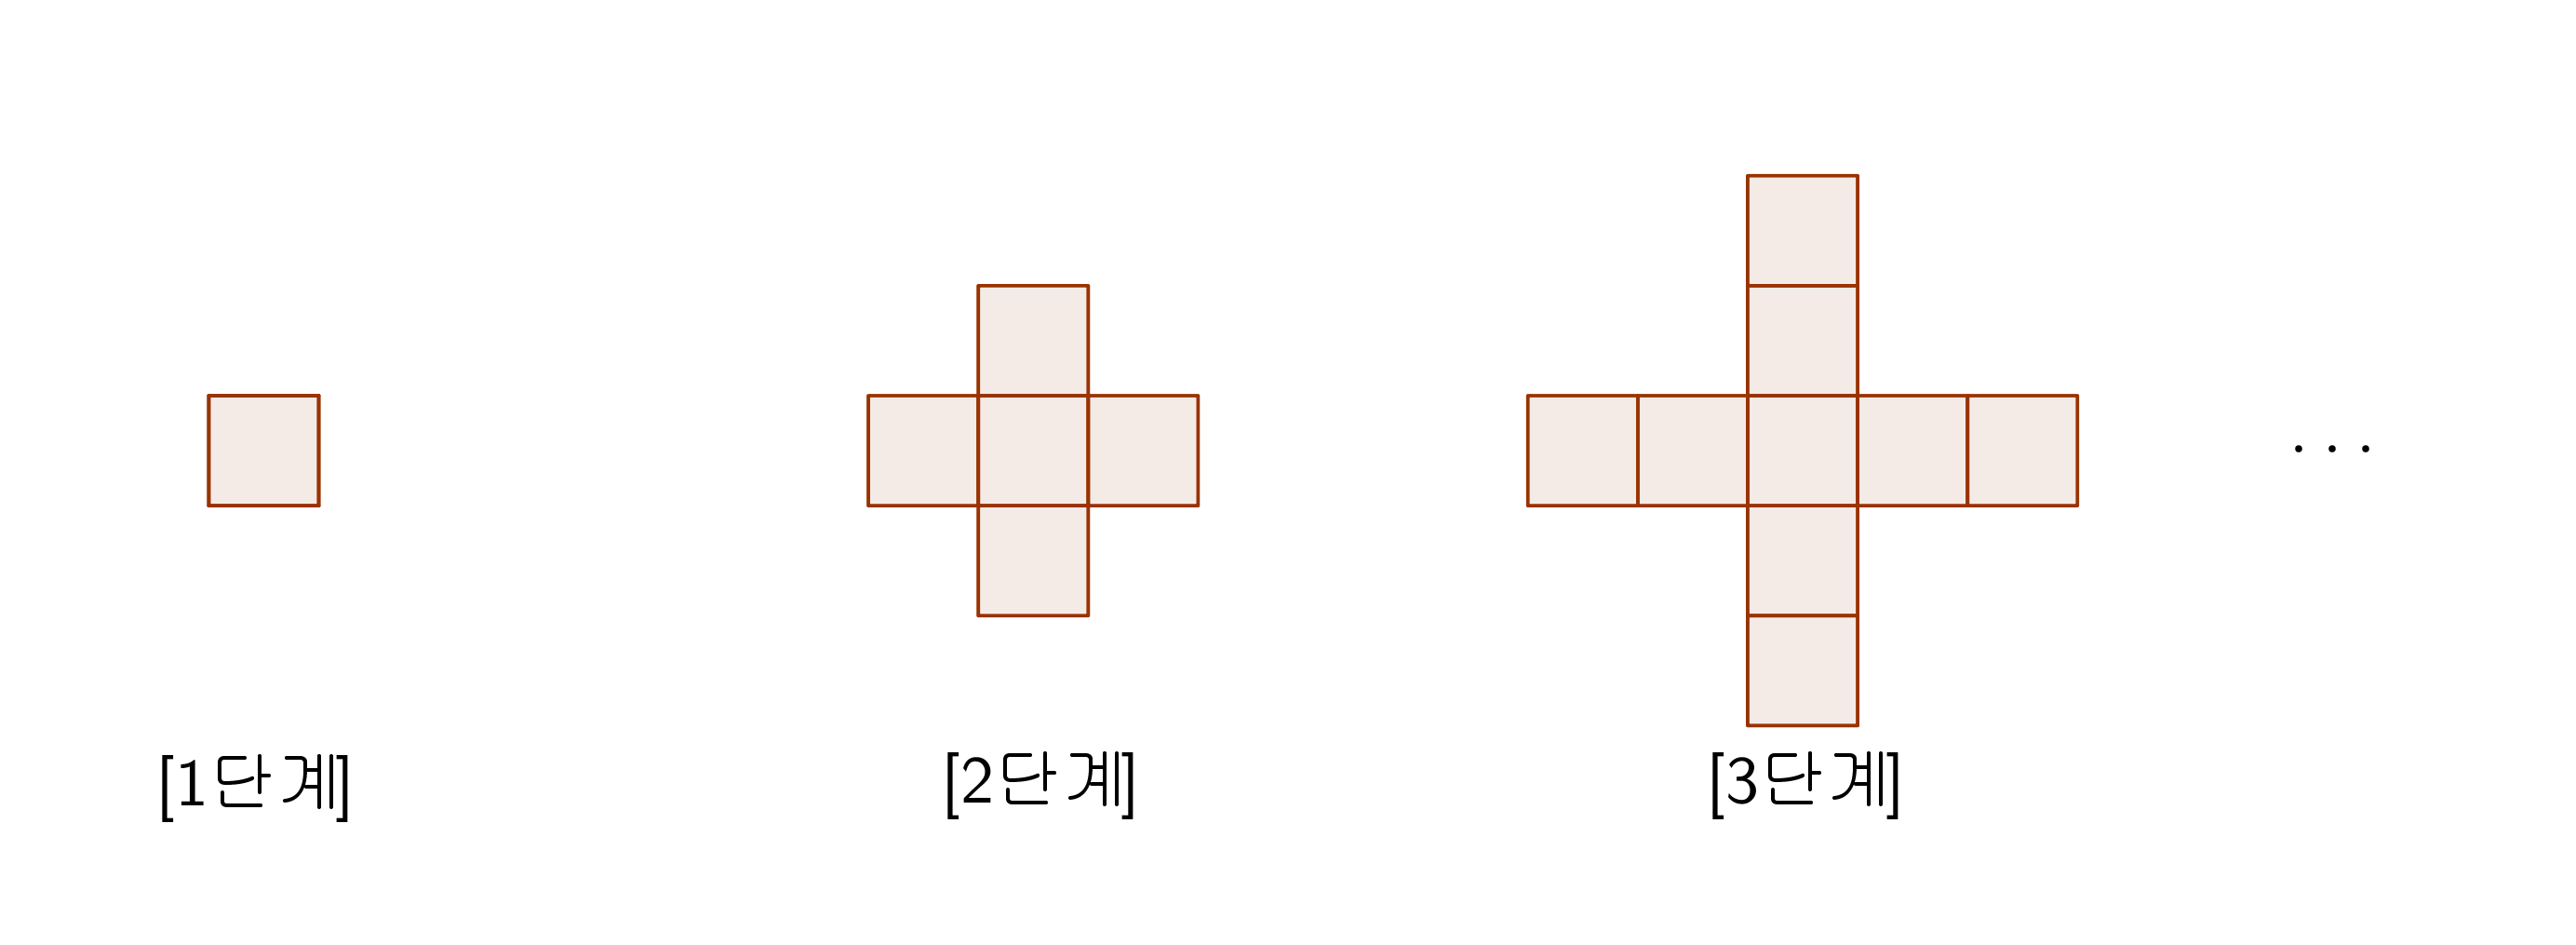
\includegraphics[width=0.5\textwidth]{cross}
\end{figure}

\begin{enumerate}
\item
\(a_1\)의 값을 구하여라.
\item
\(a_{n+1}\)과 \(a_n\) 사이의 관계식을 구하여라.
\item
\(a_n\)을 구하여라.
\end{enumerate}

\clearpage
%
\prob{}
다음은 모든 자연수 \(n\)에 대하여
\[2+2^2+\cdots+2^{n-1}+2^n=2^{n+1}-2\]
가 성립함을 수학적 귀납법으로 증명하는 과정이다.
\begin{mdframed}[skipbelow=5pt]
\begin{enumerate}[label=\emph{[\arabic*]}]
\item
\(n=\fbox{(가)}\)일 때
\[
(좌변)=\fbox{(나)},\quad(우변)=\fbox{(나)}
\]
이므로 주어진 등식은 \(n=\fbox{(가)}\)일 때 성립한다.
\item
\(n=k\)일 때 주어진 등식이 성립한다고 가정하면
\[2+2^2+\cdots+2^k=2^{k+1}-2\]
\(n=k+1\)일 때
\begin{align*}
2+2^2+\cdots+2^k+\fbox{(다)}
&=2^{k+1}-2+\fbox{(다)}\\
&=\fbox{(라)}
\end{align*}
이므로 주어진 등식은 \(n=k+1\)일 때도 성립한다.
\end{enumerate}
따라서, \emph{[1]}, \emph{[2]}로부터 주어진 등식은 모든 자연수 \(n\)에 대하여 성립한다.
\end{mdframed}
위 과정에서 (가), (나), (다), (라)에 알맞은 것을 써넣어라.

\clearpage
%
\prob{}
모든 자연수 \(n\)에 대하여 \(n^3+5n\)이 6의 배수임을 수학적 귀납법으로 증명하여라.
\vspace{0.4\textheight}

%
\prob{}
모든 자연수 \(n\)에 대하여 다음 등식이 성립함을 수학적 귀납법으로 증명하여라.
\[
1\cdot2+2\cdot2^2+3\cdot2^3+\cdots+n\cdot2^n=(n-1)2^{n+1}+2
\]
\vspace{0.4\textheight}

\kswrapfig[Pos=r]{lines}{
%
\prob{}
평면 위에 \(n\)개의 직선이 있다.
이 중 어느 두 직선도 평행하지 않고, 어느 세 직선도 같은 점을 지나지 않는다.
이 \(n\)개의 직선에 의하여 나누어지는 영역의 개수를 \(a_n\)이라고 하자.
예를 들어 오른쪽 그림에서 \(a_3=7\)이다.
다음 물음에 답하여라.}
\begin{enumerate}
\item
\(a_n\)과 \(a_{n+1}\) 사이의 관계식을 구하여라.
\item
\(a_7\)의 값을 구하여라.
\end{enumerate}

%%
\section*{답}
%
\an{4}
(1) 14\\
(2) \(\frac18\)

%
\an{5}
(1) 13\\
(2) 15\\
(3) 161

%
\an{6}
(1) 60\\
(2) 9

%
\an{8}
(1) \(a_n=5n-4\)\\
(2) \(a_n=-2n+6\)\\
(3) \(a_n=4\cdot(-2)^{n-1}\)\\
(4) \(a_n=3^{n-2}\)

%
\an{10}
(1) \(a_n=2n^2-2n+1\)\\
(2) \(a_n=2^{\frac{n(n-1)}2}\)\\
(3) \(a_n=3\times2^{n-1}-1\)

%
\an{14}
\begin{enumerate}[label=\emph{[\arabic*]}]
\item
\(n=1\)이면
\[(좌변)=1,\quad (우변)=\frac{1\cdot2}2=1\]
이므로 식 ㉠은 \(n=1\)일 때 성립한다.
\item
\(n=k\)일때 식 ㉠이 성립한다고 가정하자.
즉
\[
1+2+3+\cdots+k=\frac{k(k+1)}2
\]
을 가정하자.
\(n=k+1\)일때에 식 ㉠이 성립한다는 것을 보이기 위해 양변에 \(k+1\)을 더하면
\begin{align*}
1+2+3+\cdots+k+(k+1)
&=\frac{k(k+1)}2+(k+1)\\
&=\frac{(k+1)(k+2)}2
\end{align*}
이다.
따라서 \(n=k+1\)일 때에도 식 ㉠이 성립한다.
\end{enumerate}
\emph{[1]}, \emph{[2]}에서 모든 자연수에 대해 식 ㉠이 성립한다.

%
\an{15}
\begin{enumerate}[label=\emph{[\arabic*]}]
\item
\(n=1\)이면
\[(좌변)=1\cdot2=2,\quad (우변)=\frac13\cdot1\cdot2\cdot3=2\]
이므로 식 ㉠은 \(n=1\)일 때 성립한다.
\item
\(n=k\)일때 식 ㉠이 성립한다고 가정하자.
즉
\[1\cdot2+2\cdot3+3\cdot4+\cdots+k(k+1)=\frac13k(k+1)(k+2)\]
을 가정하자.
\(n=k+1\)일때에 식 ㉠이 성립한다는 것을 보이기 위해 양변에 \((k+1)(k+2)\)을 더하면
\begin{align*}
&1\cdot2+2\cdot3+3\cdot4+\cdots+k(k+1)+(k+1)(k+2)\\
=&\frac13k(k+1)(k+2)+(k+1)(k+2)\\
=&\frac13(k+1)(k+2)(k+3)
\end{align*}
이다.
따라서 \(n=k+1\)일 때에도 식 ㉠이 성립한다.
\end{enumerate}
\emph{[1]}, \emph{[2]}에서 모든 자연수에 대해 식 ㉠이 성립한다.

%
\an{17}
\begin{enumerate}[label=\emph{[\arabic*]}]
\item
\(n=5\)이면
\[(좌변)=2^5=32,\quad (우변)=5^2=25\]
이므로 식 ㉠은 \(n=5\)일 때 성립한다.
\item
\(n=k\)일때 식 ㉠이 성립한다고 가정하자.
즉
\[2^k>k^2\tag{㉡}\]
을 가정하자.
\(k\)는 \(5\)이상의 자연수이므로
\[k^2-2k-1=(k-1)^2-2>0\tag{㉢}\]
이다.
따라서
\[2k^2>(k+1)^2\]
이다.
이제 \(n=k+1\)일때에 식 ㉠이 성립한다는 것을 보이기 위해 ㉡의 양변에 \(2\)를 곱하면
\[2^{k+1}>2k^2\]
이다.
여기에 ㉢를 적용하면
\[2^{k+1}>2k^2>(k+1)^2\]
이다.
따라서 \(n=k+1\)일 때에도 식 ㉠이 성립한다.
\end{enumerate}
\emph{[1]}, \emph{[2]}에서 식 ㉠은 \(5\)이상의 자연수 \(n\)에 대하여 성립한다.

%
\an{18}
(1) \(39\)\\
(2) \(512\)

%
\an{19}
(1) \(\left(\frac23\right)^{19}\)\\
(2) \(\frac1{210}\)

%
\an{20}
\ding{176}

%
\an{21}
\(a_n=3n^2-3n+2\)

%
\an{22}
\(a_n=2^n+1\)

%
\an{23}
(1) \(a_n=3^{\frac{n(n+1)}2}\)\\
(2) 제 10 항

%
\an{24}
\(a_n=\frac1n\)

%
\an{25}
(1) \(a_n=2\times3^{n-1}-1\)\\
(2) \(S_n=3^n-(n+1)\)

%
\an{26}
\(a_n=4^n-1\)

%
\an{27}
(1) \(1\)\\
(2) \(a_{n+1}=a_n+4\)\\
(3) \(a_n=4n-3\)

%
\an{28}
(가) 1\\
(나) 2\\
(다) \(2^{k+1}\)\\
(라) \(2^{k+2}-2\)

%
\an{29}
\begin{enumerate}[label=\emph{[\arabic*]}]
\item
\(n=1\)이면
\(1^3+5\cdot1=6\)은 6의 배수이므로 식 ㉠은 \(n=1\)일 때 \(n^3+5n\)은 6의 배수이다.
\item
\(n=k\)일때 \(n^3+5n\)이 6의 배수라고 가정하자.
즉 \(k^3+5k\)가 6의 배수라고 가정하자.
\(n=k+1\)일때에 \(n^3+5n\)이 6의 배수라는 것을 보이기 위해 \(n\) 대신 \(k+1\)를 대입한 \((k+1)^3+5(k+1)\)을 정리하면
\begin{align*}
(k+1)^3+5(k+1)
&=(k^3+3k^2+3k+1)+(5k+5)\\
&=(k^3+5k)+3k(k+1)+6
\end{align*}
이다.
인접한 두 자연수의 곱인 \(k(k+1)\)은 2의 배수이므로 따라서 \(3k(k+1)\)은 6의 배수이다.
따라서 \((k+1)^3+5(k+1)\)도 6의 배수이다.
\end{enumerate}
\emph{[1]}, \emph{[2]}에서 모든 자연수 \(n\)에 대해 \(n^3+5n\)은 6의 배수이다.

%
\an{30}
\begin{enumerate}[label=\emph{[\arabic*]}]
\item
\(n=1\)이면
\[(좌변)=1\cdot2=2,\quad (우변)=(1-1)\cdot2^{1+1}+2=2\]
이므로 주어진 식은 \(n=1\)일 때 성립한다.
\item
\(n=k\)일때 주어진 식이 성립한다고 가정하자.
즉
\[1\cdot2+2\cdot2^2+3\cdot2^3+\cdots+k\cdot2^k=(k-1)2^{k+1}+2\]
을 가정하자.
\(n=k+1\)일때에 식 ㉠이 성립한다는 것을 보이기 위해 양변에 \((k+1)2^{k+1}\)을 더하면
\begin{align*}
&1\cdot2+2\cdot2^2+3\cdot2^3+\cdots+k\cdot2^k+(k+1)2^{k+1}\\
=&(k-1)2^{k+1}+2+(k+1)2^{k+1}\\
=&2k\cdot2^{k+1}+2\\
=&k\cdot2^{k+2}+2
\end{align*}
이다.
따라서 \(n=k+1\)일 때에도 식 ㉠이 성립한다.
\end{enumerate}
\emph{[1]}, \emph{[2]}에서 모든 자연수에 대해 식 ㉠이 성립한다.

%
\an{31}
(1) \(a_{n+1}=a_n+(n+1)\)\\
(2) \(29\)
\end{document}